\noindent
\begin{minipage}[t]{0.265\textwidth}
    \vspace{0pt}
    % Hình Cổng Gateway Arch và ghi chú ảnh
    \noindent
    \begin{minipage}[b]{8pt}
        \rotatebox{90}{\fontsize{5}{6}\selectfont\color{gray}iStock.com / gnagel}
    \end{minipage}\hspace{3pt}%
    \begin{minipage}[b]{\linewidth-11pt}
        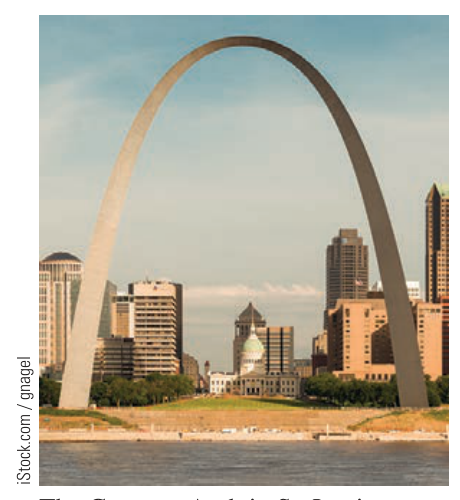
\includegraphics[width=\linewidth]{images/p0298_fig1.png}
    \end{minipage}
    
    \vskip 4pt
    \noindent{\fontsize{8.5}{10.5}\selectfont Cổng Gateway Arch ở St. Louis được thiết kế dựa trên một hàm cosin hyperbolic (xem Bài tập 56).\par}

    \vspace{24pt}
    % Hình 6: Đường tròn đơn vị
    \noindent
    \centering
    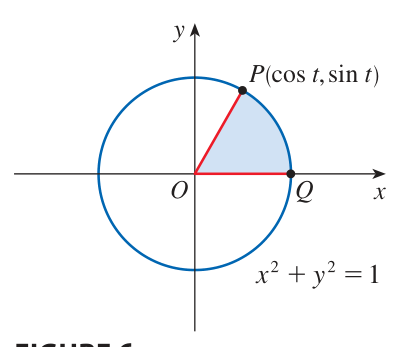
\includegraphics[width=0.88\linewidth]{images/p0298_fig2.png}
    \vskip 3pt
    {\fontsize{8.5}{10.5}\selectfont\textbf{\textsf{HÌNH 6}}\par}

    \vspace{22pt}
    % Hình 7: Hyperbol
    \noindent
    \centering
    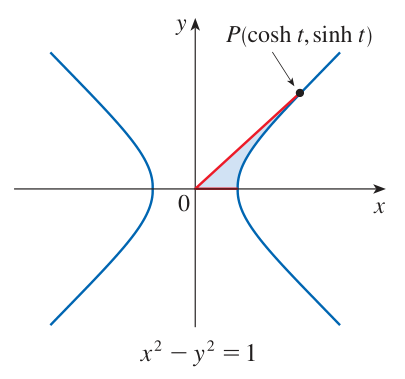
\includegraphics[width=0.88\linewidth]{images/p0298_fig3.png}
    \vskip 3pt
    {\fontsize{8.5}{10.5}\selectfont\textbf{\textsf{HÌNH 7}}\par}

\end{minipage}%
\hfill
\begin{minipage}[t]{0.70\textwidth}
    \vspace{0pt}
    \noindent\textbf{\textsf{\color{stewartcyan}VÍ DỤ 1}}\hspace{0.8em}Chứng minh rằng (a) $\cosh^2 x - \sinh^2 x = 1$ và (b) $1 - \tanh^2 x = \sech^2 x$.

    \vskip 6pt
    \noindent\textbf{\textsf{\color{stewartcyan}LỜI GIẢI}}
    \begin{align*}
    \text{(a)}\quad \cosh^2 x - \sinh^2 x &= \left( \frac{e^x + e^{-x}}{2} \right)^2 - \left( \frac{e^x - e^{-x}}{2} \right)^2 \\[5pt]
    &= \frac{e^{2x} + 2 + e^{-2x}}{4} - \frac{e^{2x} - 2 + e^{-2x}}{4} \\[5pt]
    &= \frac{4}{4} = 1
    \end{align*}

    \noindent (b) Ta bắt đầu với đồng nhất thức đã chứng minh ở phần (a):
    \[
    \cosh^2 x - \sinh^2 x = 1
    \]
    Nếu chia cả hai vế cho $\cosh^2 x$, ta nhận được
    \[
    1 - \frac{\sinh^2 x}{\cosh^2 x} = \frac{1}{\cosh^2 x}
    \]
    \noindent hay\hspace{2.5em}$1 - \tanh^2 x = \sech^2 x$\hfill{\color{stewartcyan}$\blacksquare$}

    \vskip 9pt
    \noindent Đồng nhất thức được chứng minh trong Ví dụ 1(a) đưa ra manh mối giải thích lý do cho tên gọi các hàm ``hyperbolic'':

    \vskip 4pt
    Nếu $t$ là một số thực bất kỳ, thì điểm $P(\cos t, \sin t)$ nằm trên đường tròn đơn vị $x^2 + y^2 = 1$ vì $\cos^2 t + \sin^2 t = 1$. Thực tế, $t$ có thể được hiểu là số đo bằng radian của góc $\angle POQ$ trong Hình 6. Vì lý do này, các hàm lượng giác đôi khi còn được gọi là \textit{các hàm tròn} (\textit{circular functions}).

    \vskip 4pt
    Tương tự, nếu $t$ là một số thực bất kỳ, thì điểm $P(\cosh t, \sinh t)$ nằm trên nhánh bên phải của hyperbol $x^2 - y^2 = 1$ vì $\cosh^2 t - \sinh^2 t = 1$ và $\cosh t \ge 1$. Lần này, $t$ không đại diện cho số đo của một góc. Tuy nhiên, hóa ra $t$ lại biểu thị hai lần diện tích của hình quạt hyperbol được tô màu trong Hình 7, hoàn toàn tương tự như trong trường hợp lượng giác, nơi $t$ biểu thị hai lần diện tích của hình quạt tròn được tô màu trong Hình 6.

    \vskip 4pt
    Đạo hàm của các hàm hyperbolic có thể tính toán một cách dễ dàng. Chẳng hạn,
    \[
    \frac{d}{dx}(\sinh x) = \frac{d}{dx}\left(\frac{e^x - e^{-x}}{2}\right) = \frac{e^x + e^{-x}}{2} = \cosh x
    \]
    Chúng tôi liệt kê các công thức đạo hàm cho các hàm hyperbolic trong Bảng 1. Các chứng minh còn lại được dành làm bài tập cho bạn đọc. Hãy lưu ý sự tương đồng với các công thức đạo hàm của các hàm lượng giác, nhưng chú ý rằng dấu có sự khác biệt trong một số trường hợp.

    \vskip 7pt
    % Khung Bảng 1: Đạo hàm của các hàm Hyperbolic
    \begin{tcolorbox}[
        colback=white,
        colframe=stewartred,
        boxrule=1pt,
        arc=0mm,
        left=12pt,
        right=12pt,
        top=7pt,
        bottom=8pt
    ]
        \noindent{\colorbox{stewartred}{\makebox[1.1em]{\rule[-0.2ex]{0pt}{1.8ex}\color{white}\textbf{\textsf{1}}}}\hspace{0.5em}\textbf{\textsf{\color{stewartred}Đạo hàm của các hàm Hyperbolic}}}
        \vskip 6pt
        \noindent
        \begin{minipage}[t]{0.48\textwidth}
            \begin{align*}
                \frac{d}{dx}(\sinh x) &= \cosh x \\[6pt]
                \frac{d}{dx}(\cosh x) &= \sinh x \\[6pt]
                \frac{d}{dx}(\tanh x) &= \sech^2 x
            \end{align*}
        \end{minipage}%
        \hfill
        \begin{minipage}[t]{0.48\textwidth}
            \begin{align*}
                \frac{d}{dx}(\csch x) &= -\csch x \coth x \\[6pt]
                \frac{d}{dx}(\sech x) &= -\sech x \tanh x \\[6pt]
                \frac{d}{dx}(\coth x) &= -\csch^2 x
            \end{align*}
        \end{minipage}
    \end{tcolorbox}
\end{minipage}

\vfill
\noindent
\begin{center}
    {\fontsize{6.5}{7.5}\selectfont\color{gray}
    Copyright 2021 Cengage Learning. All Rights Reserved. May not be copied, scanned, or duplicated, in whole or in part. WCN 02-200-203\\
    Due to electronic rights, some third party content may be suppressed from the eBook and/or eChapter(s).\\
    Editorial review has deemed that any suppressed content does not materially affect the overall learning experience. Cengage Learning reserves the right to remove additional content at any time if subsequent rights restrictions require it.}
\end{center}
